\chapter{图表的高级应用}
\label{chap-advanced-grammars}
\section{图表类型}
\index{Graphe!types de}\index{图表类型}
Unitex能够处理多种类型的图表,它们被用于:自动修改词典,文本预处理,文本自动机正常化,词典图表,搜索例子,消除歧义和自动图形生成。这些不同类型的图表被Unitex用不同的方式解释。某些操作,如转导,允许某些类型和禁止其他的。 此外,特殊符号是不依赖于图的类型的。本节介绍每种类型的图形及其特殊性。

\subsection{屈折图表}
\index{屈折转换器}\index{Flexion automatique}\index{Graphe!de flexion}
一个在屈折传感器通过分配屈折码来描述每个变体的形态学变化。转换器路径描述了必须应用到规范化形式和相应输出内容,包含将被创建的屈折信息。

\bigskip
\begin{figure}[!h]
\begin{center}
\includegraphics[width=4.5cm]{resources/img/fig6-1.png}
\caption{屈折语法的例子}
\end{center}
\end{figure}

\index{Opérateur!\verb+L+}
\index{Opérateur!\verb+R+}
\index{Opérateur!\verb+C+}
\index{Opérateur!\verb+D+}
\index{Opérateur!\verb+U+}
\index{Opérateur!\verb+P+}
\index{Opérateur!\verb+W+}
\index{\verb+L+}
\index{\verb+R+}
\index{\verb+C+}
\index{\verb+D+}
\index{\verb+U+}
\index{\verb+P+}
\index{\verb+W+}
\noindent 该路径可能包含运算符和字母。可能的运算符将用字符 \verb+L+, \verb+R+, \verb+C+, \verb+D+, \verb+U+, \verb+P+ et
\verb+W+.
其他所有不是运算符的字母表示字符。唯一允许的特殊符号是空词 \verb+<E>+.\index{\verb+<E>+} 我们不能在屈折转换器中参考字典中的信息,但可以引用子图。

\bigskip
\noindent 转换器的输出是连接在一起的,以产生字符串。之后字符串被添加到产生的字典条目。含有变量的输出在转换器中没有意义。


\bigskip
\noindent 字母的大小写将被保留:小写字母依旧小写,大写字母同理。此外,两个格子的连接完全等价于其内容的串联,都使输出的串联在一起。 (见例~\ref{fig-equivalent-inflection-paths}).\index{保留大小写}

\bigskip
\begin{figure}[!h]
\begin{center}
\includegraphics[width=5.5cm]{resources/img/fig6-2.png}
\caption{一个屈折语法中两条等价的路径\label{fig-equivalent-inflection-paths}}
\end{center}
\end{figure}

\bigskip
\noindent 屈折图表在被屈折项目应用前应经过编译。


\bigskip
\noindent 更多细节,见
\ref{section-automatic-inflection}.

\subsection{预处理图表}
\index{Texte!prétraitement}\index{Grammaires!pour la reconnaissance de fin de phrase}
\index{Grammaires!normalisation!de formes non ambiguës}
预处理图表被应用于被切割为词组之前的文本。这些图表被用于输入或替换文本中的片段。这种图表的两种一般用途是规范化文本,去掉歧义;以及切割句子。


\bigskip
\noindent Unitex中对这些句法图表的阐述很接近,以下是它们的区别:
\begin{itemize}
  \item 用特殊符号 \verb+<^>+ 来表示回车;\index{\verb+<^>+}
  \item 如果一个个字符的运作,我们用符号 \verb+<L>+ 表示在字母文件中定义过的一个字母;\index{\verb+<L>+}
  \item 不能在词典中用附注;
  \item 不能在词典中用形态过滤;
  \item 不能在词典中用过滤模式;
  \item 不能在词典中用上下文.
\end{itemize}

例~\ref{fig-example-sentence-splitting} (page \pageref{fig-example-sentence-splitting})
和~\ref{fig-normalization-grammar} (page \pageref{fig-normalization-grammar}) 展示了预处理图表。


\subsection{自动文本规范化图表}
\label{section-normalizing-text-automataon}
\index{Automate!du texte}\index{Texte!automate du!normalisation}
\index{Grammaires!normalisation!de l'automate du texte}
\index{Normalisation!de l'automate du texte}
\index{Normalisation!de formes ambiguës}
自动文本规范化图表能够规范化含有歧义的形式。事实上,它能描述同个形式的多个标签。这些标签随后被添加到文本中,用于明确歧义。例如~\ref{fig-tfst-normalization-grammar} 展示了规范化图表用于法语的一个摘要。

\bigskip
\begin{figure}[!h]
\begin{center}
\includegraphics[width=13.5cm]{resources/img/fig6-3.png}
\caption{规范化图表用于法语的摘要\label{fig-tfst-normalization-grammar}}
\end{center}
\end{figure}

\noindent 
路径描述需要标准化的形式。大写和小写字母遵循以下原则:在图中的大写字母在文本中自动大写;小写字母可以识别为大写和小写字母。\index{Respect de la casse}

\bigskip
\noindent 输出为标签被插入到自动文本的序列。这些标签可以是字典项或简单的字符串。标签遵循DELAF输入格式且被符号
\verb+{+ et \verb+}+分割. 变量的输出在该图表中无意义。


\bigskip
\noindent 可以调用子图表但不能在词典中添加规范化注释。在该类型图表中唯一的特殊符号是空词 \verb+<E>+.\index{\verb+<E>+}
规范化图表在被应用前应经过编译。


\subsection{句法图表}
\label{syntactic-graphs}\index{Graphe!syntaxique}\index{Grammaires!locales}
句法图表,也被称为本地语法,它可以描述能在文本中被搜索的句法模式。在所有的图表类型中,它有最大的表达能力,因为它允许参考字典。\index{Référence aux informations dans les dictionnaires}
\index{Dictionnaire!référence aux informations du}

\bigskip
\noindent 小写/大写变体根据上述原理授权。
它可以通过用引号包围短语来强制区分大小写。使用引号也可强调间距。
事实上,在Unitex的默认情况下,可以在两个格子之间加入空格。要强制空格的存在,它必须加引号。要忽略一个空格,使用特殊符号\verb+#+.\index{\verb+#+}
\index{Respect!des minuscules/majuscules}\index{Casse!voir {Respect!des minuscules/majuscules}}
\index{Minuscules!voir {Respect!de minuscules/majuscules}}
\index{Majuscules!voir {Respect!de minuscules/majuscules}}
\index{Respect!des espaces}

\bigskip
\noindent 句法图表可调用子图表。(见例
~\ref{section-subgraphs}). 它也管理输出,包括输出的变量。
生成的序列被解释为字符串,它将被插入到索引或文本如果您想改变这一个(见例
~\ref{section-modifying-text}).

\bigskip
\noindent 句法图表可使用上下文(见例~\ref{section-contexts}).

\bigskip
\noindent 句法图表可使用形态过滤器 (见例
\ref{section-filters}).

\bigskip
\noindent 句法图表可使用模式过滤器(见例
\ref{section-morphological-mode}).

\bigskip
\noindent 在句法图表中可使用的特殊符号和在关系表达式中相同 (见例~\ref{section-special-symbols}).

\bigskip
\noindent 您不必在使用之前编译语法图。如果一个图未编译,系统将自动编译它。


\subsection{语法 ELAG}
\index{Grammaires!ELAG}\index{ELAG}

本节介绍去掉歧义的句法。

\subsection{参数图表}
\index{Graphe!paramétré}
参数图表是能够产生一系列图表的图表总汇。无论哪个类型的图表都能构造为参数图表。参数图表的构造和应用将在本章中介绍~\ref{chap-lexicon-grammar}.

\section{语法的编译}
\label{section-graph-compilation}
\subsection{语法的编译}
\index{Graphe!compilation}\index{Compilation!d'un graphe}
汇编是用于将 \verb+.grf+ 格式转换为到容易由Unitex程序来处理的格式的过程。要构建一个图,您必须打开它,并从“FSGraph”菜单中单击“编译FST2”子菜单中的“工具”。
Unitex运行程序 \verb+Grf2Fst2+\index{\verb+Grf2Fst2+}\index{Programmes externes!\verb+Grf2Fst2+} ,您可以稍后在窗口中执行
(见例~\ref{fig-compilation-frame}).

\bigskip
\begin{figure}[!h]
\begin{center}
\includegraphics[width=14.7cm]{resources/img/fig6-4.png}
\caption{编译窗口\label{fig-compilation-frame}}
\end{center}
\end{figure}

\noindent 如果图表调用了子图表,子图表将被自动编译。结果是文件\verb+.fst2+ fichier\index{Fichier!\verb+.fst2+} 它集中了所有包含语法的图表。随后该语法可以被不同的Unitex程序应用。


\subsection{完成转化器}
\index{Graphe!approximation par transducteur fini}
\index{Approximation d'une grammaire par un transducteur fini}
\index{\verb+Flatten+}\index{Programmes externes!\verb+Flatten+}\label{flatten-section}
FST2格式保留了子图表的语法,转换器和完成状态间的分化。\verb+Flatten+ 程序会将一个FST2语法转换成完成状态,以及以其他方式建立一个近似值。这个特性提供了最简单的对象处理,并能自动被应用于所有的经典算法。


\bigskip
\noindent 编译和变换语法,从“FSGraph”菜单中选择“编译FST2”,从子菜单中选择“工具”。下图窗口允许您配置近似的操作。~\ref{fig-flatten-configuration}


\bigskip
\begin{figure}[!h]
\begin{center}
\includegraphics[width=10.4cm]{resources/img/fig6-5.png}
\caption{配置语法的接近\label{fig-flatten-configuration}}
\end{center}
\end{figure}

\noindent 部分“扁平化深度”用于指定子图的嵌套级别。
此值表示调用子图不会被子图本身被更换的最大深度。


\bigskip
\noindent “预期的语法模式”决定超出规定限值后程序的行为。如果您选择了“完成状态转换器”,则调用子图将超出最大深度后将被忽略。(被 \verb+<E>+ 替换)此选项可确保获得一个完成状态转换器,不等同于初始语法。另外,选项“FST2”则计划超出深度限制子图的调用。这确保了结果的与原来的语法严格等价,但不一定会产生一个完成的状态。这个选项可以用于优化某些语法。

\bigskip
\noindent 消息表明进程结束后处理的结果,如果结果是一个完成状态或一个FST2语法,且如果它等效于原始语法,在转化器中的情况。 (见例~\ref{fig-flatten-result}).


\bigskip
\begin{figure}[!h]
\begin{center}
\includegraphics[width=14.7cm]{resources/img/fig6-6.png}
\caption{Résultat de l’approximation d’une grammaire\label{fig-flatten-result}}
\end{center}
\end{figure}


\subsection{语法约束}
\index{Grammaires!contraintes}\index{Contraintes sur les grammaires}
除了屈折文法,语法不能有空路径。这意味着,一个语法主图表不能够识别空字,但是这并不妨碍该语法来识别子图。


\bigskip
\noindent 不能将输出关联到子图的调用。这类输出将被Unitex忽略。您需要用一个空框在左侧调用子图来输出。 (见例~\ref{fig-subgraph-output}).
\index{Sortie d'un transducteur!associée à un appel de sous-graphe}

\bigskip
\begin{figure}[!h]
\begin{center}
\includegraphics[width=9.1cm]{resources/img/fig6-7.png}
\caption{Comment associer une sortie à un appel de sous-graphe\label{fig-subgraph-output}}
\end{center}
\end{figure}

\index{Boucles sans fin}
\noindent 
文法不得包含无限循环。
%A void loop is a configuration that causes the \verb+Locate+ program to enter an infinite loop.
这些循环可能是由于使用空字或递归调用子图。


\bigskip
\noindent 
空字引起的循环可以有两个原因,所述第一如下~\ref{fig-epsilon-output-loop}.
这种类型的循环是因为由空字不能自动由Unitex除去。~\ref{fig-epsilon-output-loop} 因此,图中的空字不会被删除,并会导致无限循环。

\bigskip
\begin{figure}[!h]
\begin{center}
\includegraphics[width=6.2cm]{resources/img/fig6-8.png}
\caption{Boucle infinie due à une transition par le mot vide avec sortie\label{fig-epsilon-output-loop}}
\end{center}
\end{figure}

\bigskip
\noindent 第二类循环涉及到能识别空字的子图的调用。如下图:~\ref{fig-epsilon-subgraph-loop}: 若子图 \verb+Adj+ 能识别空字,则是一个无限循环。

\bigskip
\begin{figure}[!ht]
\begin{center}
\includegraphics[width=7.9cm]{resources/img/fig6-9.png}
\caption{无限循环,由于一个子图调用
\label{fig-epsilon-subgraph-loop}}
\end{center}
\end{figure}

\begin{figure}[!ht]
\begin{center}
\includegraphics[width=15.5cm]{resources/img/fig6-10.png}
\caption{无限循环,由于两个图表相互调用
\label{fig-recursive-calls-loop}}
\end{center}
\end{figure}

\noindent 无限循环的第三种可能性关于向子图递归调用。考虑 \verb+Det+ 和 \verb+DetCompose+ 在下图中~\ref{fig-recursive-calls-loop}。
这些图表可以相互调用\textit{sans rien lire dans le texte}. 事实上,这些图表既不包括初始状态也不调用其他图表 实际上,如果在图表 \verb+Det+ 和对 \verb+DetCompose+ 的调用间有不同, 意味着Unitex
 探索图表 \verb+Det+ 应该在递归调用之前阅读文本标签 \verb+DetCompose+ 在这种情况下,程序可能不能无限期地发生迭代。

\pagebreak
\subsection{重复数的间隔}
\label{nb-repetitions}\index{Intervalle}\index{Boucle!nombre de répétitions}\index{Nombre de répétitions}\index{Répétition!nombre de}
\noindent 
要区别序列中的模式出现一次多次,或者永不出现,我们可以在一个格子里一个整数范围中相关联。遵循次数的限制,图案必须在单个格子进行说明。
如果我们将区间 [m,M] 与一个包含 <A> (figure~\ref{intervals})的盒子相关联, 至少有$ M$连续形容词,且不超过$ M$更多。

\begin{figure}[h!]
\begin{center}
\includegraphics[width=13.5cm]{resources/img/fig6-10a.png}
\caption{识别若干个连续的指令\label{intervals}}
\end{center}
\end{figure}

\noindent  在格子的输出间隔插入 \verb+$[m,M]$+ ,
在符号 ``/''之后, 有以下规则 : 
\begin{itemize}
\item \verb+[m,M]+ = 至少 $m$ 连续词,不超过 $M$
\item \verb+[,M]+ = 从 0 到 $M$  
\item \verb+[m,]+ = 至少 $m$
\end{itemize}

\noindent 格子不应通过循环被连接到自身。
通常输出兼容。例如,在图中插入格子~\ref{intervals}
la sortie \verb+<ADJ 位置='antéposé'>+,在以下行文本中可知~: \verb+<A>/$[1,4]$/<ADJ position='antéposé'>+. 

\subsection{错误检测}
\index{Détection d'erreur dans les graphes}\index{Graphe!détection d'erreur}
\index{Erreurs dans les graphes}
为了防止程序阻塞或崩溃,Unitex编译图表自动执行错误检测。该编译器会检查主要内容,不承认空词并搜索所有形式的无限循环。如果发现错误,将出现在编辑窗口中显示错误消息。例~\ref{fig-error-message} 是编译\verb+Det+得到的信息~\ref{fig-recursive-calls-loop}.

\begin{figure}[!h]
\begin{center}
\includegraphics[width=15cm]{resources/img/fig6-11.png}
\caption{Message d’erreur obtenu en compilant le graphe
\texttt{Det}\label{fig-error-message}}
\end{center}
\end{figure}

\noindent 如果搜索图案为 \verb+.grf+ \index{Fichier!\verb+.grf+}搜索操作被自动中断。


\section{上下文}
\index{Contexte!zone dans un graphe}\label{section-contexts}

这些Unitex图表是代数。它们也被称为上下文无关文法,因为当一个人希望识别序列 $A$时,不考虑 $A$ 的上下文。例如,它不可能在正常的曲线,找到 \verb+president+, 
除非之后有 \verb+of the republic+。


\bigskip
\noindent Il est toutefois possible de tenir compte du contexte dans les graphes syntaxiques. Dans
ce cas, les graphes ne sont plus des grammaires algébriques, mais des grammaires contex-
tuelles qui n’ont pas les mêmes propriétés théoriques.
.

\subsection{上下文的区域}
\index{\verb+$[+}
\index{\verb+$]+}
上下文的由图表的大小及
\verb+$[+ 和 \verb+$]+ 划定。绿色方括号在图表中表示上下文的开始和结束。上下文的开头和结尾必须出现在同一张图上。

\bigskip
\begin{figure}[!h]
\begin{center}
\includegraphics[width=7.4cm]{resources/img/fig6-12.png}
\caption{上下文区域的使用\label{fig-context1}}
\end{center}
\end{figure}

\bigskip
\noindent 例~\ref{fig-context1} 显示了上下文的一个简单的例子。此图可以识别所有号码
欧元,英镑或美元,没有出现的符号,则在索引中。

\bigskip
\noindent 上下文被解释如下。假设应用语法文字注释时和 $pos$ 在文字当前位置。语法 \verb$Locate$ 随后会搜索上下文中的表达。 如果失败了,将不会运行。如果成功的话,也就是说,如果他能达到的上下文的结时,程序将返回到 $pos$ 并将从上下文的末端继续语法的探索。

\bigskip
\noindent 上下文区域 (见~\ref{Transducers}) 的权重将被忽略。

\bigskip
\noindent 你也可以定义消极上下文,使用
 \verb+$![+ 作为上下文的开始。图~\ref{fig-context2}
示出了识别之后有 \verb+th+.
 的曲线图。与正上下文找到不同的是,当\verb$Locate$试图识别的上下文中描述的表达,如到达上下文的端部被认为是失败的,因为这意味着我们承认非法序列。反之,如果不能达到上下文的结束时,\verb$Locate$程序将返回到定位位置。

\begin{figure}[!h]
\begin{center}
\includegraphics[width=7.3cm]{resources/img/fig6-13.png}
\caption{消极上下文的应用\label{fig-context2}}
\end{center}
\end{figure}

\bigskip
\noindent 上下文可以在任何地方在图中被放置,包括开头。图~\ref{fig-context3} 示出了一个图,其识别在某物的上下文是不是一个过去分词一个形容词。换句话说,该图承认所有不属于歧义与过去分词的形容词。

\begin{figure}[!h]
\begin{center}
\includegraphics[width=7.5cm]{resources/img/fig6-14.png}
\caption{用过去分词搜索无歧义形容词\label{fig-context3}}
\end{center}
\end{figure}

\bigskip
\noindent 在图表中,例如在图~\ref{fig-context3}, 中,消极上下文不一定检查相同数量的框标记。例如,在图~\ref{too-also} 之前,如果它出现在一个表达式,如 \verb+too+,消极上下文检查 \verb+too early+ 或 \verb+too many+.

\begin{figure}[!h]
\begin{center}
\includegraphics[width=7.5cm]{resources/img/fig-too-also.png}
\caption{Un contexte qui ne vérifie pas le même nombre de mots que la boite qui le suit\label{too-also}}
\end{center}
\end{figure}

\bigskip
\noindent 我们可以制定与消极权利背景复杂的查询。因此,图
~\ref{fig-context4} 显示了可识别的两个简单的名字不是歧义或复合词的所有序列图。事实上, \verb?<CDIC><<^([^ ]+ [^ ]+)$>>? 
识别包含正好一个空格的复合词 \verb?<N><<^([^ ]+)$>>?
,而图案 \textit{Black cats should like the town hall}, 图表识别了
 \textit{Black cats}, 但未识别 \textit{town hall}。

\bigskip
\begin{figure}[!h]
\begin{center}
\includegraphics[width=8.9cm]{resources/img/fig6-15.png}
\caption{上下文的先进应用\label{fig-context4}}
\end{center}
\end{figure}

\bigskip
\noindent 您可以连接上下文。例如,~\ref{fig-context5}
图表识别了后面没有一个点的数字的数量,除非这个点后是一个数字。因此,在文本 \textit{5.0+7.=12}, 图表能识别 \textit{5}, \textit{0} 和
\textit{12}.

\bigskip
\begin{figure}[!h]
\begin{center}
\includegraphics[width=12cm]{resources/img/fig6-16.png}
\caption{连接上下文\label{fig-context5}}
\end{center}
\end{figure}

\bigskip
\noindent 在一个格子内的输出将被忽略。然而,可以使用已经在上下文中定义的变量,如图 ~\ref{fig-context6})。若我们对文本
\textit{the cat is white}应用MERGE模式, 将输出 :

\bigskip
\texttt{the \textcolor{blue}{<pet name="cat" color="white"/>} is white}

\bigskip

\begin{figure}[!h]
\begin{center}
\includegraphics[width=12.2cm]{resources/img/fig6-17.png}
\caption{上下文中定义的变量\label{fig-context6}}
\end{center}
\end{figure}

\subsection{上文}
\index{\verb+$*+}
另外也可以查找表达 $X$ 若它只能在 $Y$ 后被找到。 很显然,已经可以用语法来做到这一点,如图 \ref{fig-left-context1}. 
然而,在这种类型的语法中,上文包括在识别序列中,如图~\ref{fig-left-context2}.

\begin{figure}[!ht]
\begin{center}
\includegraphics[width=7cm]{resources/img/fig6-17a.png}
\caption{通过数字开头的名称识别\label{fig-left-context1}}
\end{center}
\end{figure}

\begin{figure}[!ht]
\begin{center}
\includegraphics[width=14cm]{resources/img/fig6-17b.png}
\caption{图标号的应用的结果
\ref{fig-left-context1}\label{fig-left-context2}}
\end{center}
\end{figure}

\bigskip
\noindent 为了避免这种情况,你可以使用 \verb+$*+ 在上文的结束表示我们想要识别的词。该符号在图中用绿色的星表示,如图~\ref{fig-left-context3}. 这样的情况下的效果是使用部分语法来计算识别序列,这部分不显示结果(见图~\ref{fig-left-context4}).

\begin{figure}[!ht]
\begin{center}
\includegraphics[width=9cm]{resources/img/fig6-17c.png}
\caption{在上文识别名词\label{fig-left-context3}}
\end{center}
\end{figure}

\begin{figure}[!ht]
\begin{center}
\includegraphics[width=14cm]{resources/img/fig6-17d.png}
\caption{图表语法的应用结果
\ref{fig-left-context3}\label{fig-left-context4}}
\end{center}
\end{figure}

\clearpage
\noindent 由上文产生的所有输出将被忽略,如图 \ref{fig-left-context6}, 图表语法的应用结果被给出 \ref{fig-left-context5}.

\begin{figure}[!ht]
\begin{center}
\includegraphics[width=9cm]{resources/img/fig6-17e.png}
\caption{上文产生的所有输出将被忽略\label{fig-left-context5}}
\end{center}
\end{figure}

\begin{figure}[!ht]
\begin{center}
\includegraphics[width=15cm]{resources/img/fig6-17f.png}
\caption{图表语法的应用结果
\ref{fig-left-context5}\label{fig-left-context6}}
\end{center}
\end{figure}

\bigskip
\noindent 然而,它可存储与变量(见第
\ref{section-variables}) 的信息,并使用于上文之外,如图~\ref{fig-left-context7} 和结果~\ref{fig-left-context8}.

\begin{figure}[!ht]
\begin{center}
\includegraphics[width=10cm]{resources/img/fig6-17g.png}
\caption{上文变量的应用\label{fig-left-context7}}
\end{center}
\end{figure}

\begin{figure}[!ht]
\begin{center}
\includegraphics[width=15cm]{resources/img/fig6-17h.png}
\caption{图表语法的应用结果
\ref{fig-left-context7}\label{fig-left-context8}}
\end{center}
\end{figure}

\bigskip
\noindent 我们可以调用包含在上文的语法,但需要警惕。当上文被从所识别的序列中排除时,由调用者识别的所有序列的图形也被排除在外,因为这将最终被识别的序列必须是连续的。对应于该排除的序列的输出也被忽略。

\bigskip
\noindent 因此,在上下文中,可以划分用于识别该文本分的模式和序列的结果。例如,图 \ref{fig-left-context9} 正在查找 \verb$the animal's$,但只提取名词,因此我们可以看到图 \ref{fig-left-context10}.

\begin{figure}[!ht]
\begin{center}
\includegraphics[width=10cm]{resources/img/fig6-17i.png}
\caption{上下文语法\label{fig-left-context9}}
\end{center}
\end{figure}

\begin{figure}[!ht]
\begin{center}
\includegraphics[width=15cm]{resources/img/fig6-17j.png}
\caption{图表语法的应用结果
\ref{fig-left-context9}\label{fig-left-context10}}
\end{center}
\end{figure}

\bigskip
\noindent 权重 (见~\ref{Transducers}) 一般在上文中无作用。

\clearpage

\section{形态学方法}
\label{section-morphological-mode}
\index{形态学方法}
\subsection{为什么 ?}
Unitex的版本“tokenisée”无法接受“标记”内的查询与形态过滤器
(见 \ref{section-filters}),如图
\ref{fig-morpho1}.

\begin{figure}[!ht]
\begin{center}
\includegraphics[width=8cm]{resources/img/fig6-17k.png}
\caption{形态元素的识别\label{fig-morpho1}}
\end{center}
\end{figure}

\bigskip
\noindent 但是,形态过滤器不允许任何查询,原因是它们不能引用包含在字典信息。因而,不能执行以这种指令 ``\textit{含有后缀} \verb$un$ \verb+able+''。

\bigskip
\noindent 为了克服这个困难,我们在程序中引入一个形态模式
\verb$Locate$. 它用符号划定你的部分语法 \verb+$<+ et \verb+$>+.\index{\verb+$<+}\index{\verb+$>+}
在这个模式中,数据是由字母识别的字母,如图
\ref{fig-morpho2}.

\begin{figure}[!ht]
\begin{center}
\includegraphics[width=11cm]{resources/img/fig6-17l.png}
\caption{语法形态区的例子\label{fig-morpho2}}
\end{center}
\end{figure}

\subsection{规则}
在这个模式中,图形的内容不被正常解释。
\begin{enumerate}
\item 还有就是格子之间没有空格。因此,如果我们识别空格,就必须用 \verb+" "+ (引号间的空格).

\item 我们始终可以使用子图,但形态学区域的开始于结束必须在相同的图。

\item 与法可以咨询字典
--- 如\verb+<DIC>+ , \verb+<be>+ 或 \verb+<N:ms>+, 
只要信息包含在一个字典中,那么它作为条目 (见~\ref{dic-mode-morpho})。
   
\item 人们可以咨询一个词条
(见~\ref{section-dictionary-graphs}), 只要辞典图形的名称中包含选项 \verb+b+.
但是,此选项仅适用于由图的词典的最初应用时已识别 (见~\ref{section-applying-dictionaries}),
而不是出现在文本作为标记的部件的形式。
   
\item 我们可以使用形态过滤器 (见~\ref{section-filters}). 但是,单独使用形态滤波器或\verb+<TOKEN>+
将仅适用于当前字符。因此,该过滤器作为 \verb+<<[1-9][0-9]>>+ 被设计为不会识别多个字符。事实上,在形态学方法中形态过滤器仅用于表达否定 \verb+<<[^aeiouy]>>+ (即不是元音的任何字符). 
   
\item 上文权力的部分定义~\ref{section-contexts} 是被禁止的。

\item 我们可以使用输出。
   
\item \verb+<LETTER>+ 能识别在字母表中定义的所有字符
	\index{\verb+<MOT>+}\index{\verb+<LETTER>+}

\item \verb+<LOWER>+ 能识别在字母表中定义的小写字符。\index{\verb+<MIN>+}\index{\verb+<LOWER>+}

\item \verb+<UPPER>+ 能识别在字母表中定义的大写字符。\index{\verb+<MAJ>+}\index{\verb+<UPPER>+}

\item \verb+<DIC>+ 能识别在形态学词典中中定义的所有字符\index{\verb+<DIC>+}, 除了一些符号如 \verb+#+, \verb+<FIRST>+,  \verb+<NB>+,
 	 \verb+<SDIC>+ et\verb+<CDIC>+ sont interdits.\index{\verb+#+} \index{\verb+<FIRST>+} \index{\verb+<NB>+} \index{\verb+<TOKEN>+} \index{\verb+<SDIC>+} \index{\verb+<CDIC>+}
\item 
如果我们没有在指令的最后到达终点区,识别失败。
	例如,一个文本包含 \verb+enabled+, 我们不能只识别
	\verb+enable+.
\end{enumerate}

\noindent  一些原先的符号 \verb+<LETTER>+, \verb+<LOWER>+ 和 \verb+<UPPER>+
仍能使用 \verb+<MOT>+, \verb+<MIN>+ 和 \verb+<MAJ>+。
他们仍然运作,以保持与现有的图形系统的向后兼容性,但他们现在已经过时,也就是说,我们建议避免使用他们来设计最新版本的工作图表\footnote{从版本 3.1bêta起},不会不必要地增加在使用词条数。

\subsection{形态模式词典}
\index{形态模式词典}
\label{dic-mode-morpho}
在形态模式中,我们可以查询词典。
例如 \ref{fig-morpho3} 查找由 \verb+un+ 和形容词构成的内容。

\begin{figure}[!ht]
\begin{center}
\includegraphics[width=11cm]{resources/img/fig6-17m.png}
\caption{识别由 \textit{un} 和形容词构成的内容
\textit{able}\label{fig-morpho3}}
\end{center}
\end{figure}

\begin{figure}[!ht]
\begin{center}
\includegraphics[width=11cm]{resources/img/fig6-17n.png}
\caption{形态模式词典声明\label{fig-morpho4}}
\end{center}
\end{figure}

\bigskip
\noindent 为了能够用该语法识别
\verb+unaware+ 系统必须知道 \verb+aware+ 是一个形容词。
词法面具\verb+<A>+需要咨询字典。但是,\verb+aware+ 不存在于文本,所以你不能依靠词典\footnote.这就是为什么我们必须定义词典列表来咨询的形态模式(见~\ref{section-applying-dictionaries})。要做到这一点,进入“信息>首选项>模式形态词典”(例~\ref{fig-morpho4})。我们可以定义为许多字典,我们希望形态的方式,但他们必须在format\verb+.bin+。这一事实可应用语法。要指定一个图形的字典应该在形态模式下,使用选项\verb+b+ 或 \verb+z+(见~\ref{section-dictionary-graphs},形态字典输出方式)。



\subsection{词典变量}
\index{词典变量}
\index{形式变量}
\label{dictionary-variables}

您可以指定从字典形态模式变量的信息。
这些变量被称为变量字典或形态的变量。
该类型的变量的初始化必须含有是指包含在形态学模式字典信息的格子相关联,在\verb+<DIC>+的特例中. 我们将 \verb+$xxx$+ 输出,如果 \verb+xxx+ 是一个变量名 (见~\ref{section-using-variables})。会将一个变量重命名为 \verb+xxx+ 通过图案识别的字典条目。
在经过该框以下路径,可以得到的词尾变化的形式,规范形式和编码由与输入供给\verb+$xxx.INFLECTED$+, \verb+$xxx.LEMMA$+ 和 \verb+$xxx.CODE$+, 如
\ref{fig-morpho5}.
我们也可以使用以下方式:

\begin{itemize}
\item \verb+$xxx.CODE.GRAM$+:只提供第一个语法码,语法范畴
  
\item \verb+$xxx.CODE.SEM$+: 给出所以码,用 \verb$+$ 分隔
  
\item \verb+$xxx.CODE.FLEX$+:给出所有可变码,用 \verb$:$分隔

\item \verb+$xxx.CODE.ATTR=yyy$+ 返回包含在语义代码的属性值对的值也就是 \verb+zzz+ 和 \verb+yyy+ 是否含有以下形式的语义代码 \verb+yyy=zzz+。

\end{itemize}
	
\noindent 变量的字典可以形态学模式以外使用,例如
 \ref{fig-morpho7}. 如可以对这些变量测试 \ref{section-variables}.

\begin{figure}[!ht]
\begin{center}
\includegraphics[width=16cm]{resources/img/fig6-17o.png}
\caption{变量的字典的用途\label{fig-morpho5}}
\end{center}
\end{figure}

\begin{figure}[!ht]
\begin{center}
\includegraphics[width=15cm]{resources/img/fig6-17p.png}
\caption{在MERGE模式下的结果语法图\ref{fig-morpho5} 
\label{fig-morpho6}}
\end{center}
\end{figure}

\begin{figure}[!ht]
\begin{center}
\includegraphics[width=15.5cm]{resources/img/fig6-17q.png}
\caption{使用普通模式变量字典\label{fig-morpho7}}
\end{center}
\end{figure}


\bigskip
\noindent \textbf{Variables de dictionnaire dans LocateTfst}

\noindent 对于使用 \verb+LocateTfst+的语法 (见~\ref{section-locate-tfst}), 
它有一个附加的可能性。除了形态学模式,可以存储在包含在文本自动机的字典可变词汇的标签。只要结合形式的输出框 \verb+$:abc$+ 中 \verb+abc+
是一个变量名。

然后,您可以照常字典变量使用,如上文所述:
人们可以得到词尾变化的形式,规范形式,并在入口给出的代码,语法范畴,它的语义编码,屈折码和值
 \verb+zzz+ 和对应的 \verb+yyy+ 他们是否符合 \verb+yyy=zzz+.


\section{探索语法路径}
\index{Exploration des chemins d’une grammaire}

有可能产生由语法识别的路径,例如来检查它正确地生成预期的形式。要做到这一点,打开主图的语法和确保图形窗口是活动窗口(活动窗口有一个蓝色的标题栏,同时非活动窗口有灰色的标题栏)。然后进入菜单“FSGraph”,然后在子菜单“工具”,然后点击“浏览路径图”。窗口如下图
~\ref{fig-explore-graph-paths} 。


\begin{figure}[!h]
\begin{center}
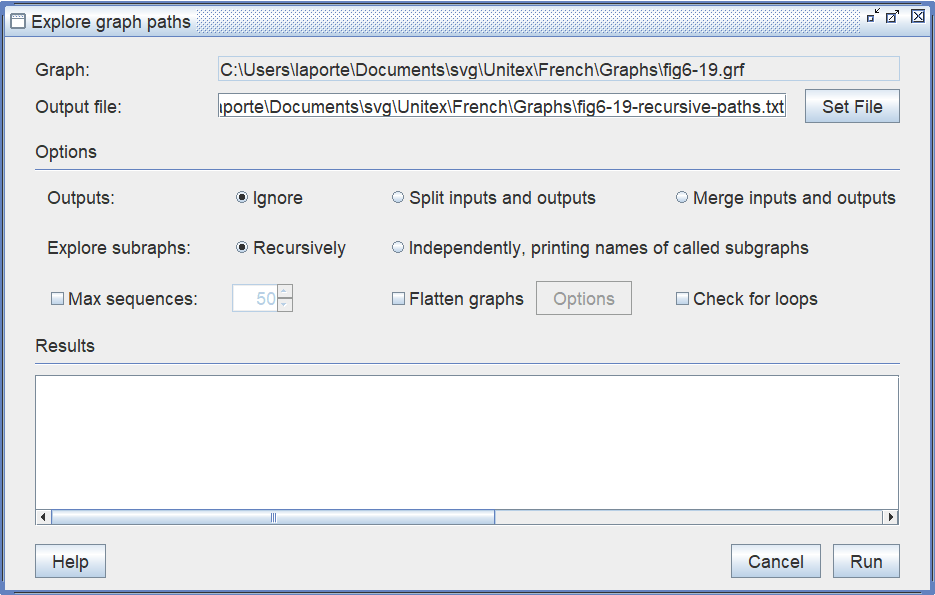
\includegraphics[width=10.4cm]{resources/img/fig6-18.png}
\caption{探索语法路径\label{fig-explore-graph-paths}}
\end{center}
\end{figure}

\bigskip
\noindent 以上包含了主要的图形语法探索路径的名字。
以下是语法和扫描模式的输出管理选项:


\begin{itemize}
  \item “忽略输出”:输出被忽略;
  \item “独立的输入和输出”:独立显示的输入和输出的条目
  (\verb$ a b c / A B C$);
  \item “合并输入和输出”:对应后立即显示每个输出
  (\verb$a/A b/B c/C$).
  \item “唯一路径”:调用子图递归探索;
  \item “不递归探索子图”:调用将正在探索递归显示在子图。
\end{itemize}

\noindent 如果“序列的最大数目”被选中,则指定的数量将所产生的路径的最大数目。如果未选择该选项,所有的路径将被产生。


\bigskip
\noindent 这就是用于曲线图中得到的 ~\ref{fig-glace} 
使用默认设置(忽略输出,限制=100条路径):


\bigskip
\noindent
\texttt{<NB> <boule> de glace \`a la pistache}

\noindent
\texttt{<NB> <boule> de glace \`a la fraise}

\noindent
\texttt{<NB> <boule> de glace \`a la vanille}

\noindent
\texttt{<NB> <boule> de glace vanille}

\noindent
\texttt{<NB> <boule> de glace fraise}

\noindent
\texttt{<NB> <boule> de glace pistache}

\noindent
\texttt{<NB> <boule> de pistache}

\noindent
\texttt{<NB> <boule> de fraise}

\noindent
\texttt{<NB> <boule> de vanille}

\noindent
\texttt{glace \`a la pistache}

\noindent
\texttt{glace \`a la fraise}

\noindent
\texttt{glace \`a la vanille}

\noindent
\texttt{glace vanille}

\noindent
\texttt{glace fraise}

\noindent
\texttt{glace pistache}

\begin{figure}[!h]
\begin{center}
\includegraphics[width=10.9cm]{resources/img/fig6-19.png}
\caption{图表举例 \label{fig-glace}}
\end{center}
\end{figure}




\section{图集合}
\index{Collection de graphes}

有时候我们希望应用在同一目录中的多个语法。对于这一点,有可能从一个文件树自动构建语法。例如,假设你有以下三种:


\begin{itemize}
  \item \textit{Dicos}:
  \begin{itemize}
    \item \textit{Banque}:
    \begin{itemize}
      \item \texttt{carte.grf}
    \end{itemize}
    \item \textit{Nourriture}:
    \begin{itemize}
      \item \texttt{eau.grf}
      \item \texttt{pain.grf}
    \end{itemize}
    \item \texttt{truc.grf}
  \end{itemize}
\end{itemize}

\noindent 如果想要把所有这些语法融入其中,你可以用“构建集图”子菜单中的“FSGraph>工具”做到这一点。它通过图1的窗口配置操作
~\ref{fig-build-graph-collection}.

\begin{figure}[!h]
\begin{center}
\includegraphics[width=9cm]{resources/img/fig6-20.png}
\caption{构建图形的集合\label{fig-build-graph-collection}}
\end{center}
\end{figure}

\noindent 
在“源目录”字段中,选择你想探索(在我们的例子中,根目录 \textit{Dicos})。在“结果GRF语法”字段中,输入所产生的语法的名称。


\bigskip
\noindent 注意:不要将输出的语法放入探索树,因为在这种情况下,该计划将同时读取和写入该文件,这将导致崩溃。

\bigskip
\noindent 当您单击“确定”按钮,程序会复制在输出语法目录中的图表,并创建对应于不同的子目录子图,如图~\ref{fig-graph-collection}。

\bigskip
\noindent 
可以看出,一个框包含此处相应于子目录子图呼叫(例 \textit{Banque}
和 \textit{Nourriture})和其他框使用目录中的图表 (见图 \texttt{truc.grf}).

\begin{figure}[!h]
\begin{center}
\includegraphics[width=11cm]{resources/img/fig6-21.png}
\caption{主图收集图表\label{fig-graph-collection}}
\end{center}
\end{figure}



\section{传感器的规则}
\label{section-applying-transducers-rules}
\index{Transducteur!règles d'application}\index{Règles!pour l'application des transducteurs}
本节介绍了在治疗前操作和搜索模式,应用传感器的规则。图表屈折和歧义形式不包含下文。


\subsection{将识别的图案插入前边}
\index{MERGE}\index{REPLACE}
当传感器被应用在替换模式,输出替换文本阅读序列。
%When a box in a transducer has no output, it is processed as if it had an \verb+<E>+ output.
在管理模式下,输出被插入到所识别的序列的左边。考虑图1的转换器~\ref{fig-transducer-example}
. 

\begin{figure}[!h]
\begin{center}
\includegraphics[width=7.2cm]{resources/img/fig6-22.png}
\caption{转换器例\label{fig-transducer-example}}
\end{center}
\end{figure}

\bigskip
\noindent 
%Look at the transducer in Figure~\ref{fig-transducer-example}.
\noindent 如果我们将此传感器应用于Sir Walter Scott的小说\textit{Ivanhoe} 
在MERGE模式下,我们得到下图~\ref{fig-transducer-example-concordance} 


\begin{figure}[!h]
\begin{center}
\includegraphics[width=14.4cm]{resources/img/fig6-23.png}
\caption{MERGE模式与图1的转换器获得的协议
~\ref{fig-transducer-example}\label{fig-transducer-example-concordance}}
\end{center}
\end{figure}

\subsection{应用推进}
在预处理,文本修改为,当它消失了。为了避免无限循环的危险,它不需要由转换器产生的序列,可以通过将其重新分析。因为这个原因,当一个序列在文中被引入,所述转换器的应用在该序列后继续进行。
这条规则只适用于预处理的转换器,因为语法图的应用过程中,输出不改变文本阅读,而是一个单独的索引文件的文本。


\subsection{左优先}
\label{section-priorite-gauche}
\index{Priorité!à la séquence de gauche} \index{Chevauchement d'occurrences}
在本地语法中,重叠出现的都是索引。我们在这里看到的真正的重叠发生为 \verb+abc+ et \verb+bcd+, 而不是 \verb+abc+ et \verb+bc+.
所有这些实例中示出(见~\ref{fig-overlappping-occurrences})。

\begin{figure}[!h]
\begin{center}
\includegraphics[width=13cm]{resources/img/fig6-24.png}
\caption{出现在相应的重叠\label{fig-overlappping-occurrences}}
\end{center}
\end{figure}

\noindent 但是,如果您编辑的文本,而不是构建一个和谐的,有必要这些事件将被考虑中进行选择。为此,Unitex应用以下优先规则:最左边的序列优先。

\bigskip
\noindent 运用这一规则,三个事件之前的情况中,发生 \textcolor{blue}{\texttt{[in ancient]}}和
\textcolor{blue}{\texttt{[ancient times]}}。因此左边保持在第一,因为它是最左边,而 \textcolor{blue}{\texttt{[ancient times]}} 被删除。下一个  \textcolor{blue}{\texttt{[times a]}} 不再被包括
\textcolor{blue}{\texttt{[ancient times]}} 可能出现在结果中:

\begin{center}
\texttt{...Don, there extended \textcolor{blue}{[in ancient] [times a]} large forest...}
\end{center}

\noindent 左优先规则只适用于当文本被修改,无论是在前处理,或之后 (见~\ref{section-modifying-text}).

\subsection{优先级更高的区段}
\index{Priorité!à la séquence la plus longue}
在一个句法图的应用是可能的选择优先级是否应给予的序列更短或更长,或者如果所有的序列应当保留。在预加工中,优先级总是被赋予较长的序列。


\subsection{变量输出}
\label{section-variables}
\index{Variable!dans un graphe}\index{Sortie d'un transducteur!avec variable}
正如我们在~\ref{section-using-variables}所看到的,它可以使用输入变量来存储,是由一个语法分析的文本。这些变量可以在预处理和在语法图形图表中使用。


\bigskip
\noindent 你必须给名称使用的变量。这些名称可以包含\verb+A+和\verb+Z+,重音大写或小写,数字和字符之间的符号\verb+_+ (下划线).\index{点}

\bigskip
\noindent 要设置开始和该区域的最终存储在一个输入变量,或使用按钮,在图表上方的图标栏的红色括号(见~\ref{toolbar-commands}),
,或者你创建两个格子,含有可变目标的名称个字符\verb-$- 和 \verb-(- 是开始区域,其他的由 \verb-$- 和 \verb-)- 为结束。
Pour utiliser une variable dans une sortie, 要在输出时使用一个变量,在之前和之后用 \verb-$-
 (voir figure~\ref{fig-variable-definition}).

\bigskip
\noindent 变量是全局性的。这意味着你可以在一个图表定义一个变量并在另一个调用它,如图所示~\ref{fig-variable-definition}. 如果我们对\textit{Ivanhoe}应用MERGE模式的\verb+TitleName+
,我们会得到下图~\ref{fig6-14}.

\begin{figure}[!p]
\begin{center}
\includegraphics[width=16cm]{resources/img/fig6-25.pdf}
\caption{在一个子图设定的输入变量\label{fig-variable-definition}}
\end{center}
\end{figure}

\begin{figure}[!p]
\begin{center}
\includegraphics[width=13.5cm]{resources/img/fig6-26.png}
\caption{通过图形的应用程序获取协议 \texttt{TitleName}\label{fig6-14}}
\end{center}
\end{figure}

\index{Déplacement de groupes de mots}
\bigskip
\noindent 变量输出可用于移动字的组。事实上,转换器REPLACE模式的应用不会写在输出文本。交换两个词组,就可以将它们存储在变量和以任何顺序执行这些变量产生输出。因此,图的转换器~\ref{fig-swapping-words}的REPLACE模式应用于\textit{Ivanhoe}将给出以下结果~\ref{fig-no-space-problem}.

\begin{figure}[!ht]
\begin{center}
\includegraphics[width=11.3cm]{resources/img/fig6-27.png}
\caption{字的反转具有两个输入变量\label{fig-swapping-words}}
\end{center}
\end{figure}

\begin{figure}[!ht]
\begin{center}
\includegraphics[width=13.4cm]{resources/img/fig6-28.png}
\caption{图的换能器的应用结果~\ref{fig-swapping-words}\label{fig-no-space-problem}}
\end{center}
\end{figure}

\bigskip
\noindent 如果一个变量的开头或结尾是未定义的(可变的前端和末端),它会被忽略输出。见 \ref{section-advanced-search-options}该错误的变量处理。

\bigskip
\noindent 对可用的变量的数目没有限制。

\bigskip
\noindent    
输入变量可以被嵌套,甚至在图重复所示~\ref{fig-overlapping-variables}.

\begin{figure}[!ht]
\begin{center}
\includegraphics[width=15cm]{resources/img/fig6-29.png}
\caption{重复输入变量\label{fig-overlapping-variables}}
\end{center}
\end{figure}

%\clearpage


\newpage

\section{输出变量}
\label{section-output-variables}
\index{Variable!de sortie}
输入变量的声明与图标栏 \verb+$xxx(+ 和 \verb+$xxx)+是红色支架, 记录输入文本的部分。它也可以存储由语法产生的输出的部分。这涉及输出变量。这些变量声明的是在图形上方图标栏中的蓝色括号图标 (见~\ref{toolbar-commands}),
 \verb+$|xxx(+ 和 \verb+$|xxx)+.
它们出现在蓝色(见图~\ref{fig-output-variables}).
这个语法被应用于 MERGE 模式,处理 \textit{Ivanhoe} 产生如下结果~\ref{fig-output-variables-concord}. 

\begin{figure}[!ht]
\begin{center}
\includegraphics[width=8cm]{resources/img/fig6-17r.png}
\caption{输出变量\label{fig-output-variables}}
\end{center}
\end{figure}

\begin{figure}[!ht]
\begin{center}
\includegraphics[width=15cm]{resources/img/fig6-17s.png}
\caption{与图1的语法获得对应~\ref{fig-output-variables}\label{fig-output-variables-concord}}
\end{center}
\end{figure}

\bigskip
\noindent 当输出变量被初始化,换能器的输出序列中相应于当前发生输出都没有发出,它们仅存储在由该操作产生的输出变量。
例如,输出 \verb+ADJ+ 和 \verb+NOUN+ ,见图~\ref{fig-output-variables}
没有被插入到输入文本的左侧~\ref{fig-output-variables-concord}.
此外,输出在存储之前被处理~: 如果格子的输出包含串,如
\verb+$A.LEMMA$+,输出变量实际上并不包含这个字符串,但与变量 \verb+A+相关。

\bigskip
\noindent 输出变量仅由语法输出产生。因此,即使在合并模式,输出变量将绝不会存储在输入文本
(图~\ref{fig-output-variables} 和 \ref{fig-output-variables-concord}).

\bigskip
\noindent 当一个框定义已经定义的变量,
\index{Variable!redéfinition} 新值将覆盖旧的。
因此,如果该变量是在一个循环设置,只是在循环之后的变量的值取决于通过循环中的最后时间。


\section{对变量的操作}
\label{section-ops-on-variables}
\subsection{变量测试}
\index{Tests sur les variables}\index{Variable!interrogation}

\noindent 可以测试的变量是否被设置或不中断当前识别,如果条件没有得到验证。这是通过在一个格子的输出插入序列\verb+$xxx.SET$+ 。因此,如果变量名为 \verb+xxx+被定义,该序列将被忽略,并继续识别,否则,识别将停止,程序返回。这适用于输入变量,输出变量和字典的变量。同样,我们可以验证一个变量没有使用 \verb+$xxx.UNSET$+。见图 \ref{fig-testing-a-variable}使用了该种测试方式。 图\ref{fig-testing-a-variable-results}给出了MERGE模式的结果。

\begin{figure}[!ht]
\begin{center}
\includegraphics[width=9cm]{resources/img/fig6-29b.png}
\caption{变量测试\label{fig-testing-a-variable}}
\end{center}
\end{figure}

\begin{figure}[!ht]
\begin{center}
\includegraphics[width=10cm]{resources/img/fig6-29c.png}
\caption{变量测试结果\label{fig-testing-a-variable-results}}
\end{center}
\end{figure}


\subsection{变量比较}
\index{Comparaison!de variables}
另外,也可以以恒定或另一个变量来比较的任何类型的变量(输入,输出,或字典)的。这是通过下面的语法在一个盒子的输出中插入的序列进行~:


\bigskip
\noindent \verb+$abc.EQUAL=xyz$+

\bigskip
\noindent 如果变量\verb+abc+ 和\verb+xyz+的值不同,可阻断语法。注意,对于变量的字典,因为它存在于字典中的词尾变化的形式(注意变体~!) 。如果想比较 \verb+abc+ 和常量 \verb+JKL+使用以下方式:

\bigskip
\noindent \verb+$abc.EQUAL=#JKL$+

\bigskip
\noindent 如果内容是用不同的还可以测试\verb+UNEQUAL+.

\bigskip
\noindent 如果你想比较忽略的变量变异的情况下,可以使用以下测试:

\bigskip
\noindent \verb+$abc.EQUALcC=xyz$+ \\
ou \\
\verb+$abc.UNEQUALcC=xyz$+

\subsection{语义搜索代码在字典中的变量}
\index{Variable!code sémantique}
我们可以在字典中搜索变量 \index{Variable!dictionary entry}
(见~\ref{dictionary-variables}) 一个 ``语义代码''~\ref{section-DELAF-entry-syntax}.
对于这一点,插入在与下面的语法格子的输出序列:

\bigskip
\noindent \verb+$abc.EQ=Conc$+

\bigskip
\noindent 如果 \verb+Conc+ 不是字典中的``语义代码'' \verb+abc+, 我们可以中断搜索。一个可以在一个可变的一个时间搜索单个码。要检查的几个代码,我们把几个格子串联。

\bigskip
\noindent 此功能用于大型语法形态图,字典,以解离成单独的格子检查代码的语法和``语义代码'',接下来,如\cite{paumier_nam_2014}, page~486.
我们通过搜索对应的变量的字典,词汇模板测试语法的代码,然后做了语义编码一样。
这离解可能加快实施图表若~:
\begin{itemize}
\item 所有图形都直接或间接来自同一主图调用,
\item 主图被编译并转化为完成转换器 (见~\ref{flatten-section}),
\item 包含词汇面具电脑格子是常见的大多数路径和那些寻找语义编码字典中的变量\footnote{以这种方式,面具使该前几个研究语义代码仅执行一次的词汇字典形态模式。
它检查该语法的代码和由相同的词汇掩模的语义代码是否,这些面具成为整个语法更普遍和它们引起更多的协商字典。}.
\end{itemize}

\section{文本应用}
\label{section-applying-graphs-to-text}
本节仅包含语法图。
\subsection{搜索配置}
要应用语法图,首先打开它,然后按 "Locate
Pattern..." 在菜单 "Text"中 或按 <Ctrl+L>. 然后,您可以通过图的窗口中配置搜索
~\ref{fig-regexp-frame}.

\begin{figure}[!h]
\begin{center}
\includegraphics[width=9cm]{resources/img/fig6-30.png}
\caption{表达式搜索窗口\label{fig-regexp-frame}}
\end{center}
\end{figure}

\index{Recherche de motifs}
\noindent 选择“图表”作为标题的一部分“的形式定位模式”,并点击“设置”按钮,选择您的图形。您可以选格式 \verb+.grf+ 或 \verb+.fst2+。 如果您的图表为 \verb+.grf+格式, Unitex开始搜索前自动编译。如果你点击“调试模式”,该协议将显示在一个窗口,在这里您可以在控制器和可识别的序列,这条路径的状态名单。见此窗口~\ref{section-debug-mode}.

\bigskip
\noindent 部分“索引”,选择识别方式:

\index{Shortest matches}\index{Longest matches}\index{All matches}
\begin{itemize}
  \item “最短匹配”为主的短序列;
  \item “最长匹配”:到更长的序列优先。这是默认模式;
  \item “全匹配”:让所有的识别的序列。
\end{itemize}

\noindent 
部分“搜索限制”,可以限制或不看一个数字出现。默认情况下,搜索被限制于前200发生。
\index{Occurrences!nombre}

\bigskip
\index{MERGE}\index{REPLACE}
\noindent 
部分“语法输出”所涉及的输出操作模式。“有输入文本合并”模式,通过插入输出产生的序列。模式“替换识别序列”可以替换所生产序列识别的序列。第三模式忽略输出。最后一个模式是默认的。

\bigskip
\noindent

在“搜索算法”,可以指定是否要使用该程序定位或LocateTfst文本自动文本搜索。默认情况下,搜索与国联作为一直到目前为止所做的定位程序来完成。如果您想使用LocateTfst,请参阅~\ref{section-locate-tfst}.

\bigskip
\noindent
一旦你设置了参数,点击“搜索”进行搜索。

%\clearpage

\subsection{高级搜索选项}
\index{Options de recherche avancées}
\label{section-advanced-search-options}
如果选择“高级选项”选项卡,可以看到图的框架 \ref{fig6-advanced-options1}.

\begin{figure}[!h]
\begin{center}
\includegraphics[width=9cm]{resources/img/fig6-advanced-options1.png}
\caption{高级搜索选项\label{fig6-advanced-options1}}
\end{center}
\end{figure}

\bigskip
\index{Sortie d'un transducteur!ambiguïté}\index{Ambigu!transducteur}
\noindent “歧义输出”选项如图所示 \ref{fig6-advanced-options2},当一个键被后跟一个字可以是一个名词或形容词时,可产生对于相同的输入序列中的两个单独的输出(转换器器被所述不明确)。

\bigskip
\begin{figure}[!h]
\begin{center}
\includegraphics[width=9cm]{resources/img/fig6-advanced-options2.png}
\caption{有歧义输出的图表\label{fig6-advanced-options2}}
\end{center}
\end{figure}

\noindent 如果我们将图表及选项"允许歧义输出''应用于以下文本 \textit{Ivanhoe},
(默认), 将得到以下结果~\ref{fig6-advanced-options3}. 正如你所看到的,是为序列生成的两个输出 \textit{the noble}.

\bigskip
\begin{figure}[!h]
\begin{center}
\includegraphics[width=8.8cm]{resources/img/fig6-advanced-options3.png}
\caption{歧义输出 \textit{the noble}\label{fig6-advanced-options3}}
\end{center}
\end{figure}

\noindent在与“禁止歧义输出”选项下,我们得到该图的协议 \ref{fig6-advanced-options4},
仅有一个任意选择的输出 \textit{the noble}.

\bigskip
\begin{figure}[!h]
\begin{center}
\includegraphics[width=9cm]{resources/img/fig6-advanced-options4.png}
\caption{唯一输出 \textit{the noble}\label{fig6-advanced-options4}}
\end{center}
\end{figure}

\index{Traitement des erreurs sur les variables}
\bigskip
\noindent “代码错误策略”选项定义的行为
\verb+Locate+/\verb+LocateTfst+当他们遇到一个包含未定义的变量输出。请注意,此设置没有任何影响,如果输出被忽略。例如,考虑图2的曲线图
\ref{fig6-advanced-options5}. 

\bigskip
\begin{figure}[!h]
\begin{center}
\includegraphics[width=9cm]{resources/img/fig6-advanced-options5.png}
\caption{一个变量 \textit{A} 被定义
\label{fig6-advanced-options5}}
\end{center}
\end{figure}

\noindent 选项“忽略错误变量”下, \textit{A} 被忽略,如同空内容,见下图
\ref{fig6-advanced-options6}. 

\bigskip
\begin{figure}[!h]
\begin{center}
\includegraphics[width=12cm]{resources/img/fig6-advanced-options6.png}
\caption{变量 \textit{A}被定义
\label{fig6-advanced-options6}}
\end{center}
\end{figure}


\noindent 在“错误退出”选项下, \verb+Locate+/\verb+LocateTfst+
发出错误消息,如图 \ref{fig6-advanced-options7}.

\bigskip
\begin{figure}[!h]
\begin{center}
\includegraphics[width=9cm]{resources/img/fig6-advanced-options7.png}
\caption{输出不正确的变量\label{fig6-advanced-options7}}
\end{center}
\end{figure}

\noindent 随着“返回错误变量”选项,
\verb+Locate+/\verb+LocateTfst+ 停止探索语法。因此,变量充当削减路径,开关的功能。例如以下语法的应用
\ref{fig6-advanced-options5}只输出形容词,见如下例子 \ref{fig6-advanced-options8}. 

\bigskip
\begin{figure}[!h]
\begin{center}
\includegraphics[width=13cm]{resources/img/fig6-advanced-options8.png}
\caption{反向不正确的变量\label{fig6-advanced-options8}}
\end{center}
\end{figure}



\subsection{整合}
\index{Concordance}
搜索结果是一个包含发现所有出现的位置索引文件。图的窗口~\ref{fig-configuration-display-occurrences}展示了整合结构,修改及比较了之前的文本。


\bigskip
\index{Contexte!concordance}\index{Tri!de concordance}
\noindent 要查看比赛,你必须点击“整合”按钮。您可以设置上下文的大小。还可以选择的分类模式将被应用到所述协议中的条例,“排序”菜单。有关协议的参数的更多详细信息,请参见~\ref{section-display-occurrences}.

\bigskip
\begin{figure}[h]
\begin{center}
\includegraphics[width=10cm]{resources/img/fig6-31.png}
\caption{控制显示
\label{fig-configuration-display-occurrences}}
\end{center}
\end{figure}

\noindent 该协议是以HTML文件的形式产生
\index{Fichier!HTML} 您可以设置 Unitex 到对应被读取使用Web浏览器(见~\ref{section-display-occurrences}).\index{Navigateur web}

\bigskip
\noindent 如果你在 Unitex 的窗口中查看词,您可以点击这里访问在文本识别的序列。如果文本窗口不是图标化,文本不是太长要显示,你会看到选择的序列 (见图~\ref{fig-back-to-text}).

\bigskip
\begin{figure}[h]
\begin{center}
\includegraphics[width=13.5cm]{resources/img/fig6-32.png}
\caption{在文本中选择一个事件\label{fig-back-to-text}}
\end{center}
\end{figure}

\noindent 此外,如果文本自动机建,而不是图标化相应的窗口,点击的出现选择包含该实例句子的自动机。


\subsection{文本更改}
\label{section-modifying-text}
\index{Texte!modification}\index{Modification du texte}
您可以选择,而不是编辑构建和谐的文本。只需选择图的窗口下的“修改文本”的文件名
~\ref{fig-configuration-display-occurrences}.这个文件的扩展名必须为 \verb+.txt+.
\index{Fichier!\verb+.txt+}

\bigskip
\noindent 如果你想改变当前的文本,选择文件 \verb+.txt+。
如果您选择不同的文件名,当前的文本将不会受到影响。点击“GO”按钮,开始编辑文本。此操作期间施加的优先权规则,见~\ref{section-applying-transducers-rules}.

\bigskip
\noindent 
一旦这样做,所得到的文件是在其中输出被考虑到的文本的副本。操作标准和切成令牌被自动应用到文本文件。现有文本词典都没有改变。所以,如果你选择改变当前的文本,更改将立即生效。然后你可以在新的文本进行研究。


\bigskip
\noindent 注意:如果您选择使用您的图形忽略了出口,所有出现的情况会从文本中删除。


\subsection{提取事件}
\index{Extraction des occurrences}\index{Occurrences!extraction}
您可以提取其中包含的任何事件文本的所有句子。
要做到这一点,选择一个输出文件名与在“提取单位”“设置文件”按钮 (例~\ref{fig-configuration-display-occurrences})。
然后点击“提取匹配单位”按钮或“提取不匹配的单位”,这取决于您是否想要提取的句子中包含与否。



\subsection{词的比较}
\label{section-comparing-concordances}
\index{Comparaison!de concordances}\index{Concordance!comparaison}\index{Programmes
externes!\verb+ConcorDiff+}
\index{\verb+ConcorDiff+}

在“协议差异”比较与之前的协议的差异,如果一致。为此,该计划建成
\verb+ConcorDiff+ 文本中的优先级,然后比较它们。其结果是一个HTML页面来交替显示两条索引,留下一个空行,两个事件中仅有一个一个发生(例~\ref{fig-concordiff}).

\begin{figure}[h]
\begin{center}
\includegraphics[height=10cm]{resources/img/fig6-33.png}
\caption{对应的比较实例\label{fig-concordiff}}
\end{center}
\end{figure}

\bigskip
\noindent 
早先协议的线被隐藏,突出那些目前的协议。
在每一行中,只有识别的序列被着色。人们可以点击打开该位置的文本。

\bigskip
\noindent 蓝色表示的序列。红色指示已识别序列,但具有不同的扩展,也就是说,在两个序列重叠部分的承认。绿色表示出现在竞争中出现的序列。

\bigskip
\noindent 如果没有事先约定,该按钮被禁用。

%\clearpage
\subsection{调试模式}
\label{section-debug-mode}
当在窗口中使用 \verb+Locate+ 菜单~\ref{fig-regexp-frame}如果调试模式被激活,"定位形式",竞争是在一个特殊的窗口中 (见图~\ref{fig-debug-mode}),被分隔为三个部分:

\begin{figure}[h]
\begin{center}
\includegraphics[height=9.5cm]{resources/img/fig6-34.png}
\caption{在调试模式下注册窗口\label{fig-debug-mode}}
\end{center}
\end{figure}

\medskip 
\indent 在右上方是整合窗口。它是相同的,其中所述识别的序列显示为蓝色的正常窗口。

\medskip
\indent 右下是所使用的图形 \verb+Locate+.

\medskip
\indent 在左边,有分成三列的表:“变量”,“输出”和“匹配”。每个标记出现在“匹配”一栏,“变量”列指示框已被识别的内容,如果它有出口,会被列在“输出”。

\bigskip
\noindent 对于每一个被识别的序列,点击时,表格将被更新。如果你点击一个表行,系统将给图表中的相应框添加颜色。我们可以看到在自动识别它的文本识别的每个实例。在红色上的格的顶部的数字表示的量该格已经被识别的文本序列的数目。

\bigskip
\noindent 当应用在调试模式下图的菜单 \verb+Text>Locate Pattern+,
系统在 \verb+fst2+文件FST2在一个特殊的正式调试模式,这是不符合CASSYs兼容。参见~\ref{graphs-for-cassys} 。
